\documentclass[a4paper,UKenglish]{report}
\usepackage[utf8]{inputenc}
\usepackage{algorithm}
\usepackage{amsmath}
\usepackage[noend]{algpseudocode}
\usepackage{babel,csquotes,duomasterforside}
\usepackage{listings}
\usepackage{wrapfig}
\usepackage{graphicx}
\usepackage[backend=biber,
	    style=numeric,
	    citestyle=numeric]{biblatex}

\addbibresource{references.bib}

\usepackage{xcolor}

\usepackage{caption}
\usepackage{subcaption}
\colorlet{punct}{red!60!black}
\definecolor{background}{HTML}{EEEEEE}
\definecolor{delim}{RGB}{20,105,176}
\colorlet{numb}{magenta!60!black}

\lstdefinelanguage{json}{
	basicstyle=\normalfont\ttfamily,
    numbers=left,
    numberstyle=\scriptsize,
    stepnumber=1,
    numbersep=8pt,
    showstringspaces=false,
    breaklines=true,
    backgroundcolor=\color{background},
    literate=
     *{0}{{{\color{numb}0}}}{1}
      {1}{{{\color{numb}1}}}{1}
      {2}{{{\color{numb}2}}}{1}
      {3}{{{\color{numb}3}}}{1}
      {4}{{{\color{numb}4}}}{1}
      {5}{{{\color{numb}5}}}{1}
      {6}{{{\color{numb}6}}}{1}
      {7}{{{\color{numb}7}}}{1}
      {8}{{{\color{numb}8}}}{1}
      {9}{{{\color{numb}9}}}{1}
      {:}{{{\color{punct}{:}}}}{1}
      {,}{{{\color{punct}{,}}}}{1}
      {\{}{{{\color{delim}{\{}}}}{1}
      {\}}{{{\color{delim}{\}}}}}{1}
      {[}{{{\color{delim}{[}}}}{1}
      {]}{{{\color{delim}{]}}}}{1},
}
\title{Group creation in a collaborative P2P channel allocation protocol}
\subtitle{Identifying connected groups of access points}
\author{Hans Jørgen Furre Nygårdshaug}

\begin{document}
\duoforside[dept={Institutt for informatikk},
  program={Informatikk: programmering og nettverk},
  long]

\tableofcontents
\chapter{Disposition} 
\section {Introduction part}
\begin{itemize} 
	\item Introduction to the wifi interference problem
	\item Taking a step back and looking at other attempts on solving the problem
	\item Begin presenting Torleiv and Magnus work, the idea, and maybe the p2p protocol.
\end{itemize}

\section {Main thesis part}
\subsection{Group allocation algorithm} 

\begin{itemize} 
	\item The problem.
	\item Possible solutions? References.
	\item Complexity, out of scope for thesis. Assume problem is solved.
\end{itemize} 
\subsection{The algorithm itself} 
\begin{itemize} 
	\item Elaborating on the problem, introducing the first algorithm suggestion.
	\item Explain simulation data creation with stochastic uniform distribution.
	\item Show how the group creation algorith was created, design decisions (iterations etc).
	\item Results with visualizations through the visualization tool. 
	\item Evaluate results and consider improvements. How will this work in the wild?
	\item Introduce SSB data, the data format and why it is relevant. How is the tool made.
	\item Same procedure with result visualization and result evaluation. Do we still need improvements?
	\item Introducing Wigle as data source. Show results on map?
\end{itemize}

\section {Concluding part}
\begin{itemize} 
	\item Have we created a meaningful algorithm that can be implemented in hardware?
\end{itemize}

\clearpage
\chapter{Introduction}
\section{Channel allocation} 
To deal with the problem of channel allocation we will think of an AP as a vertex in a graph. When an AP scans its radio
it can hear the strength of all nearby wireless networks measured in dBm (decibel milliwatts). This decibel value will be
the value of the edge between one AP to another. With a graph expressing the wireless network topology, the problem
of optimally distributing channels between APs boils down to a graph coloring problem. The number of colors in the color problem,
represents the number of non-overlapping channels in 802.11. Exactly how an algorithm can be designed to optimally distribute channels within the
interfering topology is out of the scope of this thesis. However we can define some invariants that has to be true
for such an algorithm to work:
\begin{enumerate} 
	\item All APs has to run the same algorithm
	\item All APs must run the algorithm on the same connected group
	\item Because of the complexity of the problem the algorthm must solve, the number of APs in the connected group can not be too big
\end{enumerate}

Point 1 is trivial to solve or mitigate, as only APs running the algorithm will actively participate in the channel selection. A simple way to make sure that the
same algorithm is used, is by having a software version that is consistently checked with the other APs in the connected group.

Point 2 and point 3 is will be the main focus of the rest of the master thesis, as these are not so easily solved.

We can define a wireless topology graph as a set of wireless APs that are grouped together and share information about their neighbours and interference levels.
This set is what will now on be referred to as a \textit{connected group.} All members of the connected group will be considered when running the channel assignment algorithm.
For the connected group to have an actual impact on the quality of a network connection, it has to consist of nodes that normally disturbs each other substantially.

An ideal example of a connected group is an apartment builiding. The channel allocation protocol lets APs share information about who-disturbs-who the most in the building.
Then each AP can run the channel allocation algorithm. Because they run it on the same graph, every AP will find the same optimal channel distribution throughout the building,
and then switch to the correct channel. 

Even though an apartment building is most likely an optimal delimination of a connected group, in reality creating such a group is a bigger challenge. As the whole channel allocation
protocol is based on decentralized peer-to-peer technology, and no centralized server with access to demographical and geographical divisions exists, the protocol will
have to discover suitable connected groups on its own. Moreover, when the group is created the protocol will have to replicate data so that
all participants of the group has all the data required to perform channel allocation. It will also need a way to make sure that the image of the current group
is consistent within all APs in the connected group. 
\chapter{Connected groups}
To enable collaborative channel allocation, it is important for every AP to know which APs it is collaborating with.
One way to share information about who collaborates with who, is to let the access points group together. Information relevant for channel
allocation can then be shared freely within the group, between APs.

We will proceed by looking at some of the requirements for a group creation algorithm. It should work decentralized in a distributed fashion.
Hence, not only does the APs have to be imposed group membership, but they also have to be able to create and definine meaningful groups on their own.
Later we will propose an algorithm to create groups, and then evaluate computed groups based on the algorithm.


\section{Definition}
A connected group is a set of access points that are within close geographical range. The group should consist of APs that
interfere with each other when their channels are overlapping, so that overlap can be avoided with a channel allocation algorithm run within the group.
Not all APs in the connected group will necessarily be able to hear each other on the radio directly,
but all nodes should be able to hear each other through a transitive relation (neighbour of a neighbour, etc.).

\section{Requirements and assumptions}
We are going to be looking at how APs can organize themselves without a central coordinator,
but it should be noted that the creation of groups could potentially be easier if a centralized entity had the full picture of APs and their radio readings.
It could then combine geographical information along with AP readings to create consistent groups.
We will consider the two options against each other later on, but proceeding ahead with P2P group creation as the main concern. 
Essentially this means that an AP has no other knowledge of the world than the other APs it can hear on its radio.
For the sake of creating and evaluationg a group creation algorithm, we will assume a number of things that will have to be in solved at a later point:
\begin{enumerate}
	\item All APs visible on any AP's radio also runs the group creation algorithm.
	\item If an AP can see another AP on its radio, it also knows how to directly contact the AP (e.g. via TCP).
	\item All APs in a group are completely synchronous, and always have an equal image of the state of the group. 
\end{enumerate}

\section{Proposing an algorithm}\label{algorithm}
With the definition of a connected group in place, and the assumptions and requirements accounted for, we can begin proposing an algorithm.

Henceforth we will for the sake of simplicity be referring to APs that are running the group algorithm as \textit{nodes}.

Each node begins by identifying itself as a member of a group that only contains itself. Let us call it group $a$. The node shares all of
its radio readings with the rest of the members in group $a$. Group $a$ looks at all the radio readings of every member, and picks the node with the highest dBm value
to contact. Of course in the beginning there is only one node in group $a$, so this node's radio readings alone will decide which group to merge with. 

The neighbour node that has the highest dBm value is in group $b$, and this is the most crucial node to collaborate with. Hence the group $a$ merges its own group together
with the group of neighbour $b$. This happens in the following way: the members of the two groups exchange information about all their member nodes and their radio readings.
The data is now identical for all the members of both groups, and they can make identical choices, hence they are now in the same group. 

If the number of members $n$ exceeds a predefined threshold $memberThresh$ after a merge, the group should begin kicking out members from the group, starting with the node
that influences the rest of the group the least. 

To prevent the group from oscillating between kicking out members and rejoining members, once it reaches
its maximum size it should be locked for further merges. 

\section{Simulation data} \label{simdata}

\subsection{Requirements for data creation}
Before implementing and testing the group creation algorithm, we need to gather usable data to perform testing on.
The data consists of the topology size, and where on the topology a node is located. There are two ways we can get this knowledge.

The first way is creating our own data, and either assume the location of nodes,
or randomly distribute them on a topology.

The second way is getting real world data from a data source, where the topology would represent a section of a map, and the nodes would be APs,
most likely located in the households of the map.
Either way, the represenation of the topology should be the same. 

The testing data should be a set of nodes that has two coordinates $x$ and $y$ on a two-dimensional grid. Henceforth we will call the grid 
the node topology, or just the topology. When the nodes are placed on the
grid, we can compute which nodes it can hear on the radio, and add these to the nodes neighbour list. This list contains the
names of all the nodes it can hear, and how loud it is heard measured in $-dBi$. Additionally
the following parameters should be variable depending on each test scenario:
\begin{itemize}
	\item Topology size, variable width of x- and y-axis.
	\item Number of nodes
	\item Minimum distance between nodes (in meters)
	\item Minimum loudness measured in $-dBi$ for a node to account another node as a neighbour
\end{itemize}

\subsection{Program design}
The topology generation program consists of two main functionalitites.

The first functionality is being  be able to create a topology and generate nodes which are uniformly
and randomly positioned on the network topology. The size of the topology, the number of nodes and the minimum distance
between nodes are properties that can be given as input arguments to the program. 

The second functionality is computing which nodes can hear each other. We are assuming all nodes
are transmitting with equal strength, and that the environment is flat and obstacle free. 
All the neighbouring nodes that can be heard by a node, is added to its list of neighbours, and it stores the $-dBi$ value so it later can be shared with
the group. 

The resulting program, written in Python 3\cite{Python3}, contains an importable \textit{topology class}. This way, for further testing we can use different data sources to get the positions of nodes,
and only let the topology class compute the list of neighbours. 

The interference levels between APs is calculated by iterating through all the nodes. For each node $N$ we record its x and y position,
and then start a second iteration through the nodes. For each node $n$ in the second iteration we calculate the distance $d$ in
meters between $N$ and $n$ using Euclidean distance. Knowing the the distance between the nodes,  we can use the formula for free space path loss \cite{FSPL} to compute the $-dBI$ values.

For the sake of cross compatibility with other applications, the result of the computation represented in json. A topology consists of as
many JSON node-objects as there are nodes.


\subsection{Data output and visual representation} \label{simulationrep}
The following illustrates the node structure, and is an example of how a node with two neighbours will look: 

\begin{minipage}{\linewidth}
	\begin{lstlisting}[language=json]
	1: {
		"posX": 100,
		"posY": 100, 
		"ssid": "NODE1",
		"neighbourCount": 2, 
		"neighbours": {
			0: {
				"ssid": NODE2,
				"dbi": -77.23
			},
			1: {
				"ssid": NODE3,
				"dbi": -79.52
			}
		}
	}
	\end{lstlisting}
\end{minipage}

We can run the program in the following way
\begin{verbatim}./GenerateTopology.py -n 200 -w 100 -h 100 --space 10 --dbi 85 \end{verbatim}
Which instructs the program to create a topology with 200 nodes. 
The topology should be 100 by 100 meters large, and there should be at least 10 meters
between each node. The $dbi$ parameter makes sure that only nodes which can be
heard with a $-dBi$-value of $-85$ or larger should be considered neighbours.

The output is a 3.8 MB large file containing the resulting topology-data in JSON.

By writing a simple JavaScript browser application meant to interpret the output, we can
visually represent the nodes on a grid, and the result will look like what can be seen in figure \ref{fig:randtop}

\begin{figure}
	\center
	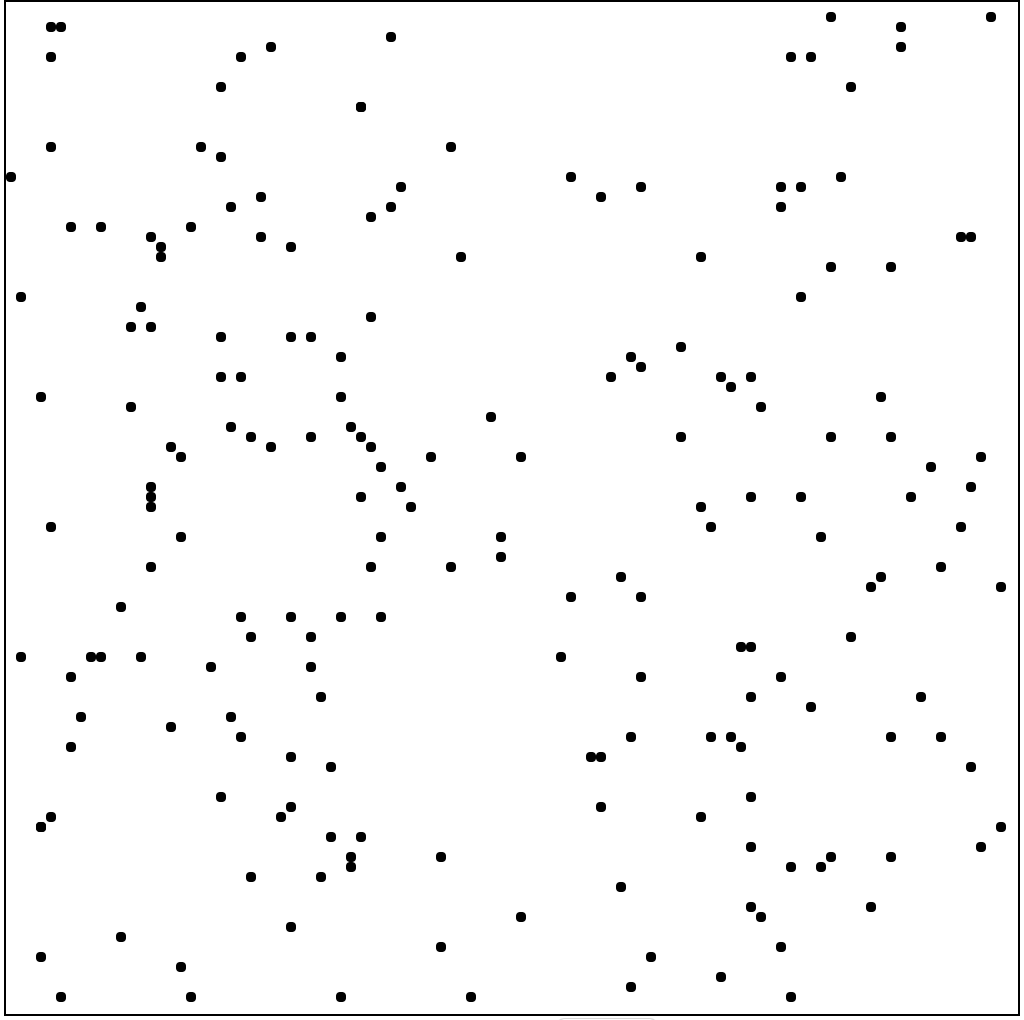
\includegraphics[scale=0.4]{Images/randomtopology.png}
	\caption{Generated topology with random, uniform distribution}
	\label{fig:randtop}
\end{figure}

\section{Algorithm implementation}
The algorithm was implemented in Python 3 \cite{Python3}, designed to run on the output from 
the data generation program.

For this computation, we are assuming that all members of a group are precicely synchronized
and the group members are consistent across all nodes. With that assumption, we can be sure
all nodes will make the same decisions. 

A group object can then be responsible for keeping track of current members,
represented as node objects. The group object will also look through the radio readings
of all its member nodes to find new member candidates, handle merges, locking the group and
kicking out extraneous members, all according to the algorithm description in section
\ref{algorithm}.
   

To make it easier to evaluate the results, the computation is done sequentially
and in iterations. This is a simple way to make sure the same groups are created
for the same topology every time, and it will make the evaluation process easier. 

The group creation program outputs a JSON-file containing the groups and their members for every iteration. The first iteration being every node having a group for their own,
and the last iteration is the resulting groups.
\section{Results}
\subsection{Uniformly distributed nodes}
We will look at how groups were created in different topology scenarios. 
All topologies presented in this section was created by the topology generation program,
but with different input parameters. Groups are distinguished by node color, where nodes
of the same color represents members of the same group. 
\subsubsection{Scenario 1}
Computed with 200 nodes with a maximum of 128 members in each group.

As can be seen in figure \ref{fig:200_128} the algorithm divides the nodes in two
sections. For clarity, a divisive line has been drawn around each group,
in case colors are not available.
When two major groups merged, the biggest groups surpasssed 128 members and began
kicking out members. The excess members formed the black group at the bottom. 

\begin{figure}
	\center
	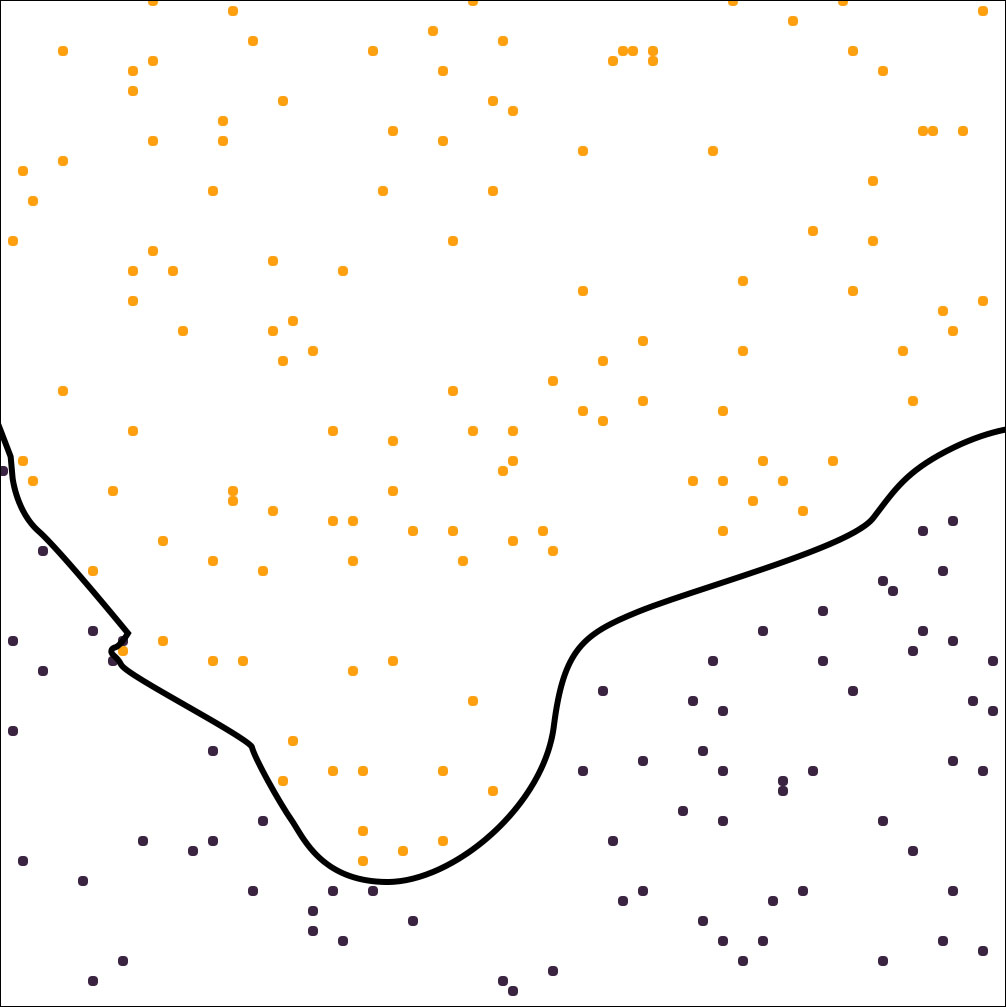
\includegraphics[scale=0.45]{Images/grouptest_1.jpg}
	\caption{200 nodes, $memberThresh=128$, $size=200x200$}
	\label{fig:200_128}
\end{figure}


\subsubsection{Scenario 2} \label{scen2}
Computed with 200 nodes with a maximum of 10 members in each group.

The result of this computation, seen in figure \ref{fig:200_10}, is a little less obvious.
The groups are again distinguished by different color, but for clarity we add a gray connecting
blob for nodes in the same group. Also blobs connected with a line are in the same group. 

It is worthy to take notice that one group is especially scattered around the graph.
At first eyesight, it looks like an algorithm deficiency, but the reason is quite simple:
when nodes are kicked out of a group during a merge, they will connet to other nodes
that belong in a group where $n$ has not yet reached $memberThresh$. When this have happened a couple of times, everyone has found a group except for the remaining few.
These are typically straggler nodes or smaller clusters separated from the others.
They are not big enough to reach the group $memberThresh$ on their own, so the merge with other
nodes that are in unmaxed groups. Thus, even though they have neighbours which
influence them more, they can only merge with nodes further away,
because that is the only unlocked group that remains.
\begin{figure}
	\center
	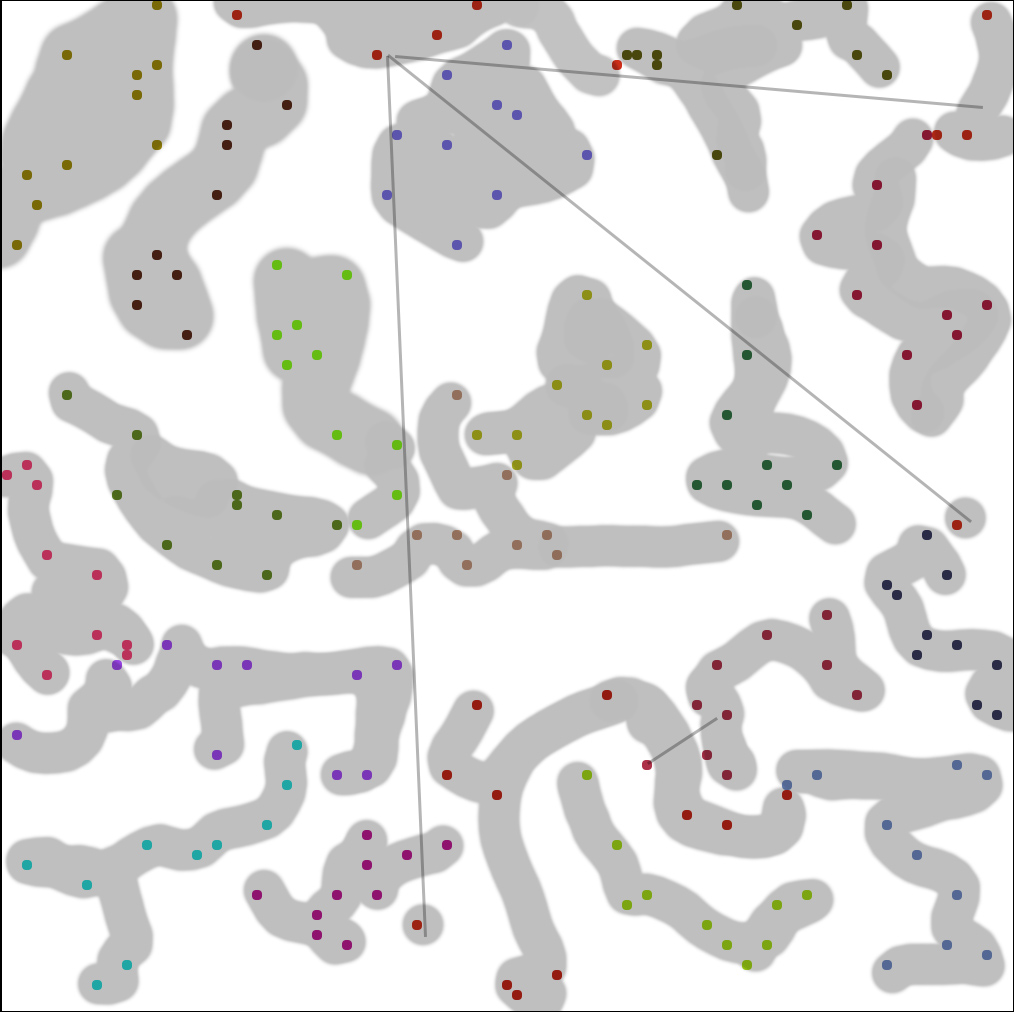
\includegraphics[scale=0.45]{Images/grouptest_2.jpg}
	\caption{200 nodes, $memberThresh=10$, $size=200x200$}
	\label{fig:200_10}
\end{figure}

\subsubsection{Scenario 3}
Computed with 5000 nodes, with a maximum for 64 members in each group. 

Figure \ref{fig:2000_64} shows the result of the computation. Because of the quantity
of nodes and the clear separation of groups, they are easily distinguished by color.
This topology is much denser than the others, and can vaguely resemble the density of highly populated areas.

We can clearly see that the overall tendency is that groups are formed
in concentrated areas of nodes. However, some groups are scattered, sometimes
all over the map. An example of a scattered group is highlighted
in figure \ref{fig:2000_64}. Its  member nodes has a thicker black line around them. 
\begin{figure}
	\center
	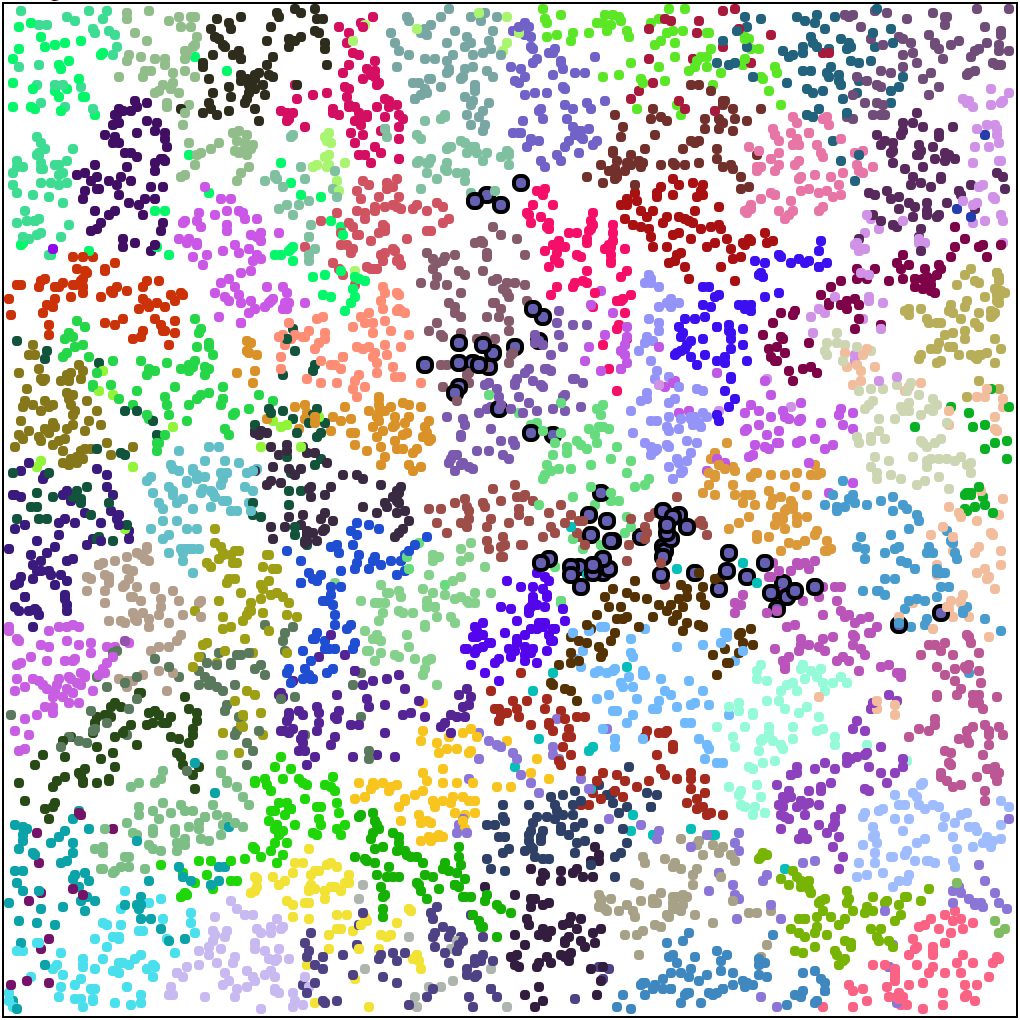
\includegraphics[scale=0.45]{Images/scenario3alt.png}
	\caption{5000 nodes, $memberThresh=64$, $size=2000x2000$}
	\label{fig:2000_64}
\end{figure}






%
%\begin{figure}
	%\centering
	%\begin{minipage}{.6\textwidth}
	%	\center
	%	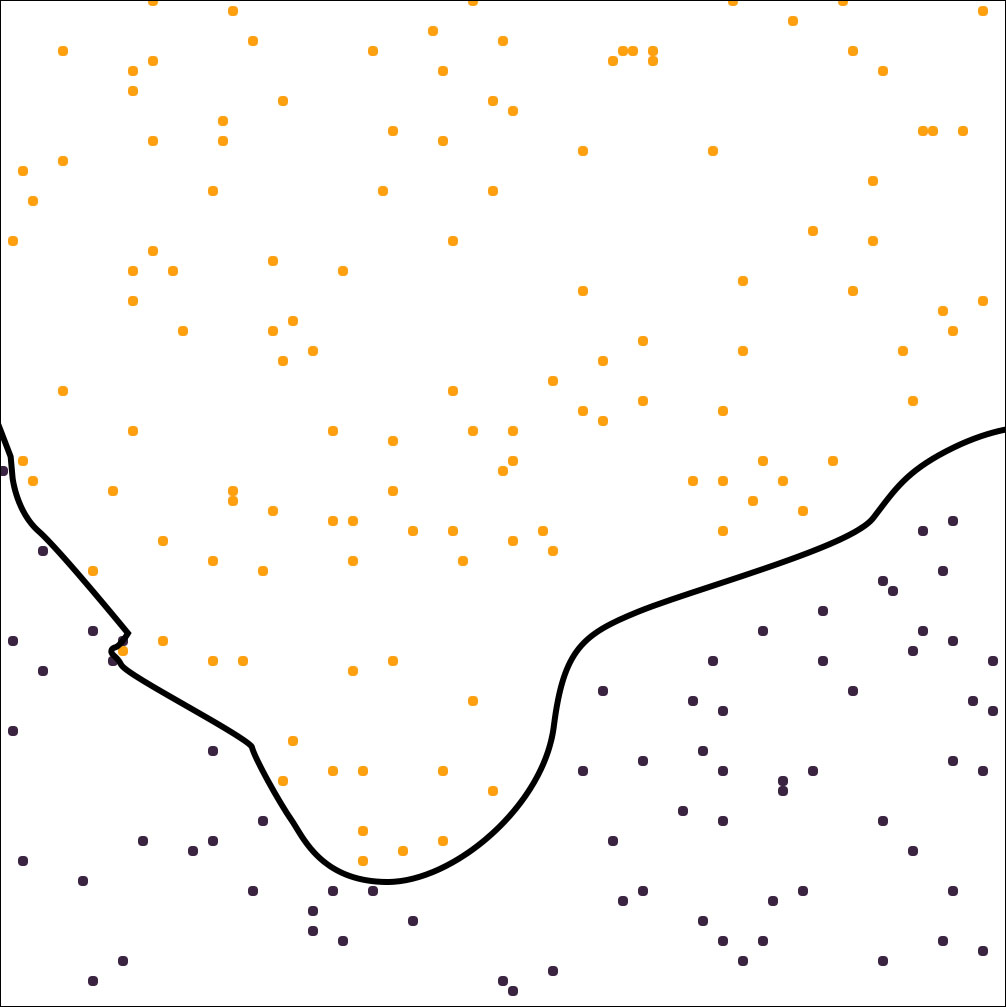
\includegraphics[width=0.9\linewidth]{Images/grouptest_1.jpg}
	%	\captionof{figure}{\newline200 nodes, $memberThresh=128$}
	%	\label{fig:200_128}
	%\end{minipage}%
	%\begin{minipage}{.6\textwidth}
	%	\center
	%	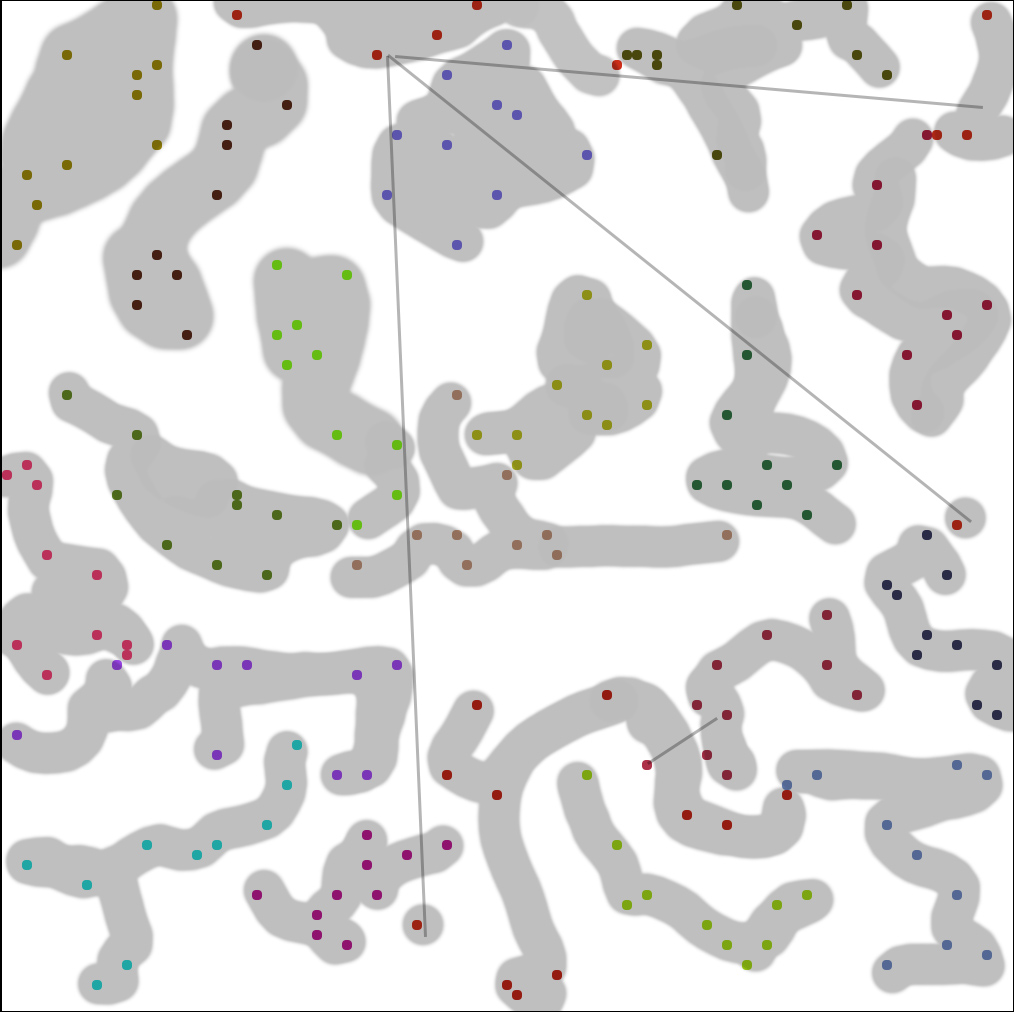
\includegraphics[width=0.9\linewidth]{Images/grouptest_2.jpg}
	%	\captionof{figure}{Another figure}
	%	\label{fig:test2}
	%\end{minipage}
%\end{figure}




\section{WiGLE}
WiGLE (Wireless Geographical Logging Engine) \cite{wigle} is a project started in 2001
which purpose is to gather information about wireless networks. The data they have
accumulated in their database is entirely user submitted. Anyone can download an 
Android app  published by WiGLE, and then use the app for wardriving
\footnote{Wardriving means tracking wireless networks using a laptop or a phone,
and then store the information about each network \cite{Wardriving}.},
then submit the data to WiGLE's centralized database. All the APs can be viewed on an interactive
map provided on WiGLE's website. The data can also be accessed through an API call.
Using their service is entirely free, but the amount of data
that can be requested is throttled on a day-to-day basis. As they openly support
research projects, they provided us with an account with a slightly higher daily data
limit.

To us this is interesting because we can use the location of APs to
create more realistic network topologies, and see how well the algorithm 
performs on these. 
 

\subsection{REST API}
Their REST API provides data presented in JSON, and offers different services,
such as user profile operations, statistical information and network search.

We only need to use the networks search part of the API for our purpose. 
By passing it a request for nodes between two latitudes
and longitudes, the API responds with the APs in that area.  
A request will look something like this: 
\begin{lstlisting}[breaklines]
https://api.wigle.net/api/v2/network/search?first=0&latrange1=37.808469&latrange2=37.746744&longrange1=-122.539232&longrange2=-122.381355
\end{lstlisting}
The parameters $latrange1$ and $longrange1$ are the coordinates that marks the beginning 
of the area we are interested in, where $latrange2$ and $longrange2$ marks the end. 
As WiGLE at most returns information about 100 APs for every query, we need the $start$
parameter to tell WiGLE at which index offset we want to begin fetching data from.
A start value of $0$ means we fetch in the range $0-99$, a value of $100$ means in the
range $100-199$ and so on. The JSON response for a succesful request for an AP,
can be seen in figure \ref{fig:wigle}.

\begin{figure}
	\begin{minipage}{\linewidth}

	\begin{lstlisting}[language=json]
{
	"userfound": false,
	"qos": 0,
	"comment": null,
	"lastupdt": "2015-12-22T17:49:34.000Z",
	"bcninterval": 0,
	"dhcp": "?",
	"lasttime": "2015-12-22T17:49:15.000Z",
	"trilong": 10.82792618,
	"netid": "5C:9E:FF:2B:54:84",
	"freenet": "?",
	"trilat": 62.2816925,
	"name": null,
	"firsttime": "2015-12-22T20:55:01.000Z",
	"type": "infra",
	"ssid": "NETGEAR23",
	"paynet": "?",
	"wep": "2",
	"transid": "20151222-00207",
	"channel": 52
}

	\end{lstlisting}

\label{fig:wigle}
	\end{minipage}
	\caption{REST API response with AP data}
\end{figure}

We are primarily interested in the properties $trilong$ and $trilat$, which is
the triangulated coordinates of the AP. 

\subsection{Using the data}
WiGLE provides data about the location of access points. However, to be able to
use the data for our group computation, we must translate the global coordinates
to two dimensional coordinates. We can then place each AP on a topology with the
same format as the generated topologies we created in section \ref{simdata}.
This is necessary for two reasons.

The first reason is that creating a group creation program that can operate
on the longitudes and latitudes directly adds more complexity. Both with regards to
group computation and visual representation. 

The second reason is that the WiGLE data does not contain information about
which neighbours each AP can hear, and with what $-dBi$ strengths they are heard.
This will have to be computed like earlier, and by parsing it to the format
we designed in section \ref{simulationrep} we can reuse the code to generate the neighbour lists.

The haversine formula [[ref or explain]] gives us the distance in meters between two coordinates. By calculating
the distane between the latitude startpoint and the latitude endpoint, we can get the size of one
axis in meters. By computing the distance between the longitude start and endpoint we get the size of the
other axis. To place a node correctly in the coordinate system, we simply use the haversine formula on the
origin coordinates to compute the distances between each axis. 

All of this has been implemented in a python program. As input it takes both latitude and longitude start and end coordinates,
then fetches all nodes within that range and inserts them on a plane. 

\section{Results}
By running the scripts that parses data from Wigle on populated areas, we should get an idea 
on how the algorithm performs in more realistic topologies. We will have a look at three
scenarios where the group allocation data is based on AP-data. 

Three suitable locations has been selected to perform the testing on Lillehammer (Norway)
a smaller city, Tynset (Norway) a less densely populated area, 
and Forks (Washington, United States). All tests were 
ran with a maximum group size of 128, and a $-dBi$ threshold of $-80$. 

\subsubsection{Lillehammer}
\begin{figure}
	\center
	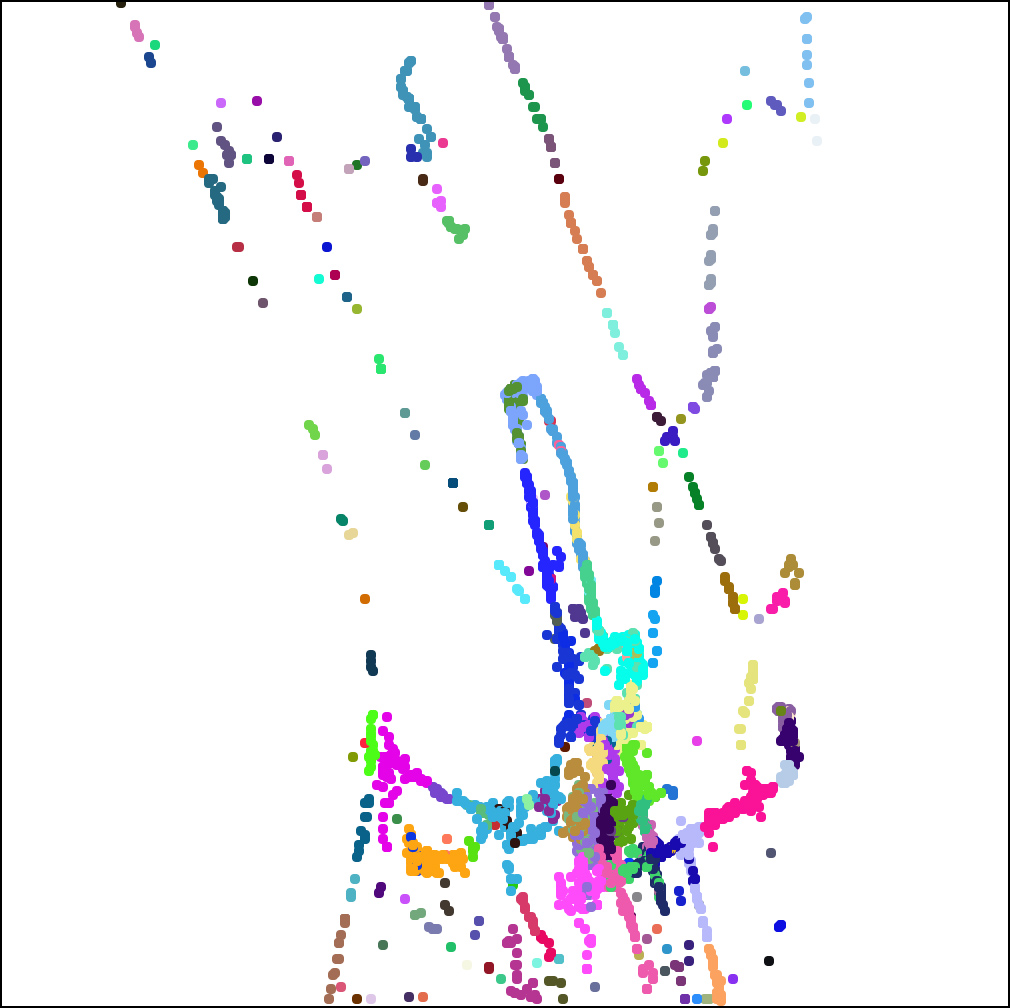
\includegraphics[scale=0.46]{Images/cities/lillehammer_groups.jpg}
	\caption{Lillehammer}
	\label{fig:lillehammer_topo}
\end{figure}

The computation results of Lillehammer can be seen in figure \ref{fig:lillehammer_topo}.
The topology is of medium density, consisting of 4990 APs, and is 2572 meters high 
and 8418 meters wide. From the tight clusters in the middle it is easy to make out the city centre.
We can clearly see different groups with different sizes. Some of the smallest groups
are highly likely so small because the distance to other nodes is too high for
the group to hear. In the denser areas they are occasionally very
entangeled, and it can be hard to make out the group borders.

Another thing to notice is that APs are nearly always placed in straight lines.
The straight lines are roads, and as Wigle collects data based on triangulation, the nodes
that is only seen once will get the position they are observed in, and not an actual
triangulated position. 
\subsubsection{Tynset}
	The computation results of Tynset can be seen in figure \ref{fig:tynset_topo}. 
	The topology consists of 726 APs, is 1670 meters high and  6720 meters wide. 
	Unsurprisingly it resembles Lillehammer on a smaller scale.
	Again we see
	some very clearly defined groups, but in the city centre there are groups
	which overlaps. We can also see nodes that are alone in their group,
	because they are too far away from anyone else.
	Much like Lillehammer, this topology is also strongly affected by the weak
	triangulation of the APs, so most APs seems to be placed on top of a road. 

\begin{figure}
	\center
	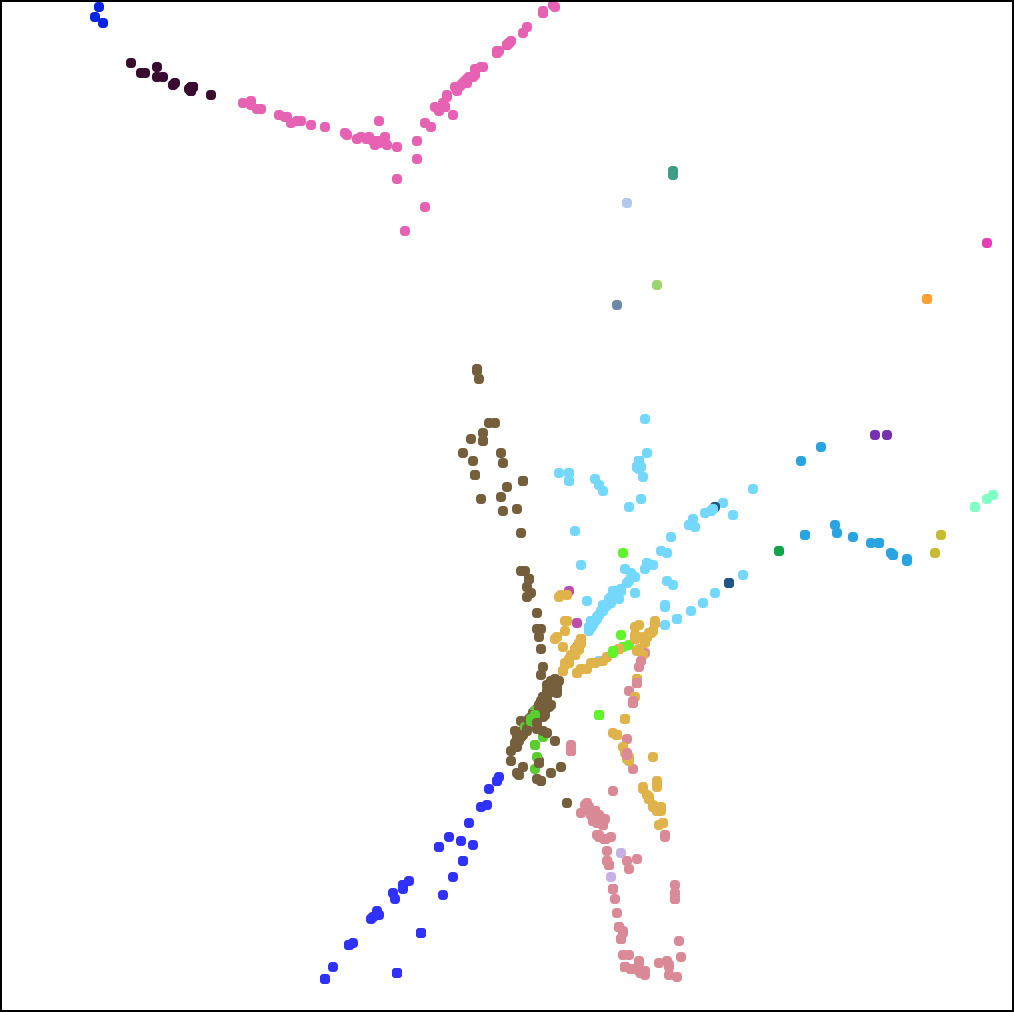
\includegraphics[scale=0.46]{Images/cities/tynset_groups.jpg}
	\caption{Tynset}
	\label{fig:tynset_topo}
\end{figure}

\subsubsection{Forks}
	
 The computation results of Forks can be seen in figure \ref{fig:forks_topo}. 
 The topology consists of 1715 nodes, and is 2122 meters high and 4495 meters wide. It
 is important to include, because it is quite different from the other topologies and
 represents a variation from the typical town and city structure of Norway.
 The size of the groups are a little more uniform when comparing it to the others.
 This can explained by the the smaller area the town is contained within. When a group
 is not full, it will almost always hear someone that it can merge with.
 We still have groups overlapping each other in the denser regions in Forks as well. 
 What is worth noticing is that the APs are positioned more realistically as locations
 of households. American towns looks more like a grid with roads in between households,
 which makes triangulation easy and a lot more accurate. 

\begin{figure}
	\center
	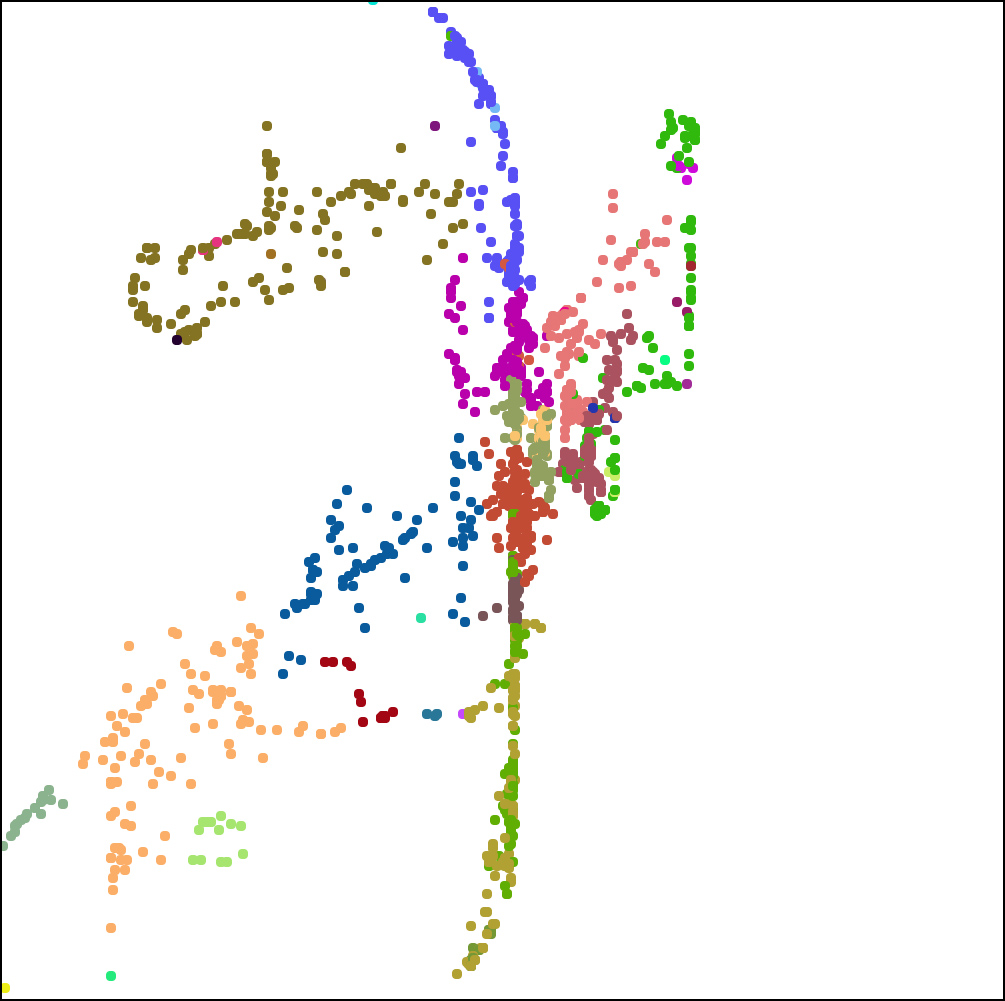
\includegraphics[scale=0.46]{Images/cities/forks_groups.jpg}
	\caption{Forks}
	\label{fig:forks_topo}
\end{figure}









%
%\makeatletter
%\def\BState{\State\hskip-\ALG@thistlm}
%\makeatother
%\subsection{Pseudocode}
%\begin{algorithm}
	%\caption{Connected group}\label{congroup}
	%\begin{algorithmic}[1]
	%\Procedure{MergeGroup}{}
	%		\State $\textit{members} \gets \text{1}$
	%		\State $i \gets \textit{patlen}$
	%		\If {$i > \textit{stringlen}$} \Return false
	%		\EndIf
	%		\State $j \gets \textit{patlen}$
%			\If {$\textit{string}(i) = \textit{path}(j)$}
%			\State $j \gets j-1$.
%			\State $i \gets i-1$.
%			\EndIf
%			\State $i \gets i+\max(\textit{delta}_1(\textit{string}(i)),\textit{delta}_2(j))$.
%			\State \textbf{goto} \emph{top}.
%		\EndProcedure
%	\end{algorithmic}
%\end{algorithm}



\printbibliography
\end{document}
